\chapter{Memerikan Sistem Kimia: Kemajuan Reaksi, Aktivitas, Q, dan K}\label{ch:b1:extent-q-and-k}

Sebuah pabrik hidrogen mengalirkan gas alam dan uap air ke dalam
tabung-tabung yang dipanaskan sampai merah membara; yang keluar tidak
pernah hidrogen murni, melainkan campuran hidrogen, karbon monoksida,
karbon dioksida, metana yang tidak bereaksi, dan uap air, yang
perbandingannya harus diketahui para insinyur sebelum merancang unit
berikutnya. Meramalkan komposisi yang keluar dari sebuah reaktor ---
keadaan akhir sebuah sistem kimia --- adalah pokok bahasan bab ini.
Untuk itu diperlukan deskripsi sistem yang tepat (variabel-variabel dan
komposisinya), satu bilangan yang mengukur seberapa jauh sebuah reaksi
telah berlangsung (\omterm{def:b1:extent-q-and-k:extent}{kemajuan reaksi}), dan hukum yang menyatakan di mana
reaksi itu berhenti (tetapan kesetimbangan). Alat-alat ini dipakai dalam
setiap bab sesudahnya tentang larutan.

\begin{recall}
Buku 1 (kelas 10) mengikuti sebuah reaksi dengan tabel kemajuan dan
menemukan \omterm{def:b1:extent-q-and-k:max-extent}{pereaksi pembatas}; Buku 1 (kelas 12) memperkenalkan \omterm{def:b1:extent-q-and-k:quotient}{kuosien
reaksi} $Q$ dan tetapan kesetimbangan $K$ reaksi yang tidak tuntas. Dari
fisika kita memakai hukum gas sempurna $pV = nRT$, dengan $R =
\qty{8.314}{J/(mol.K)}$.
\end{recall}

\begin{omfigure}
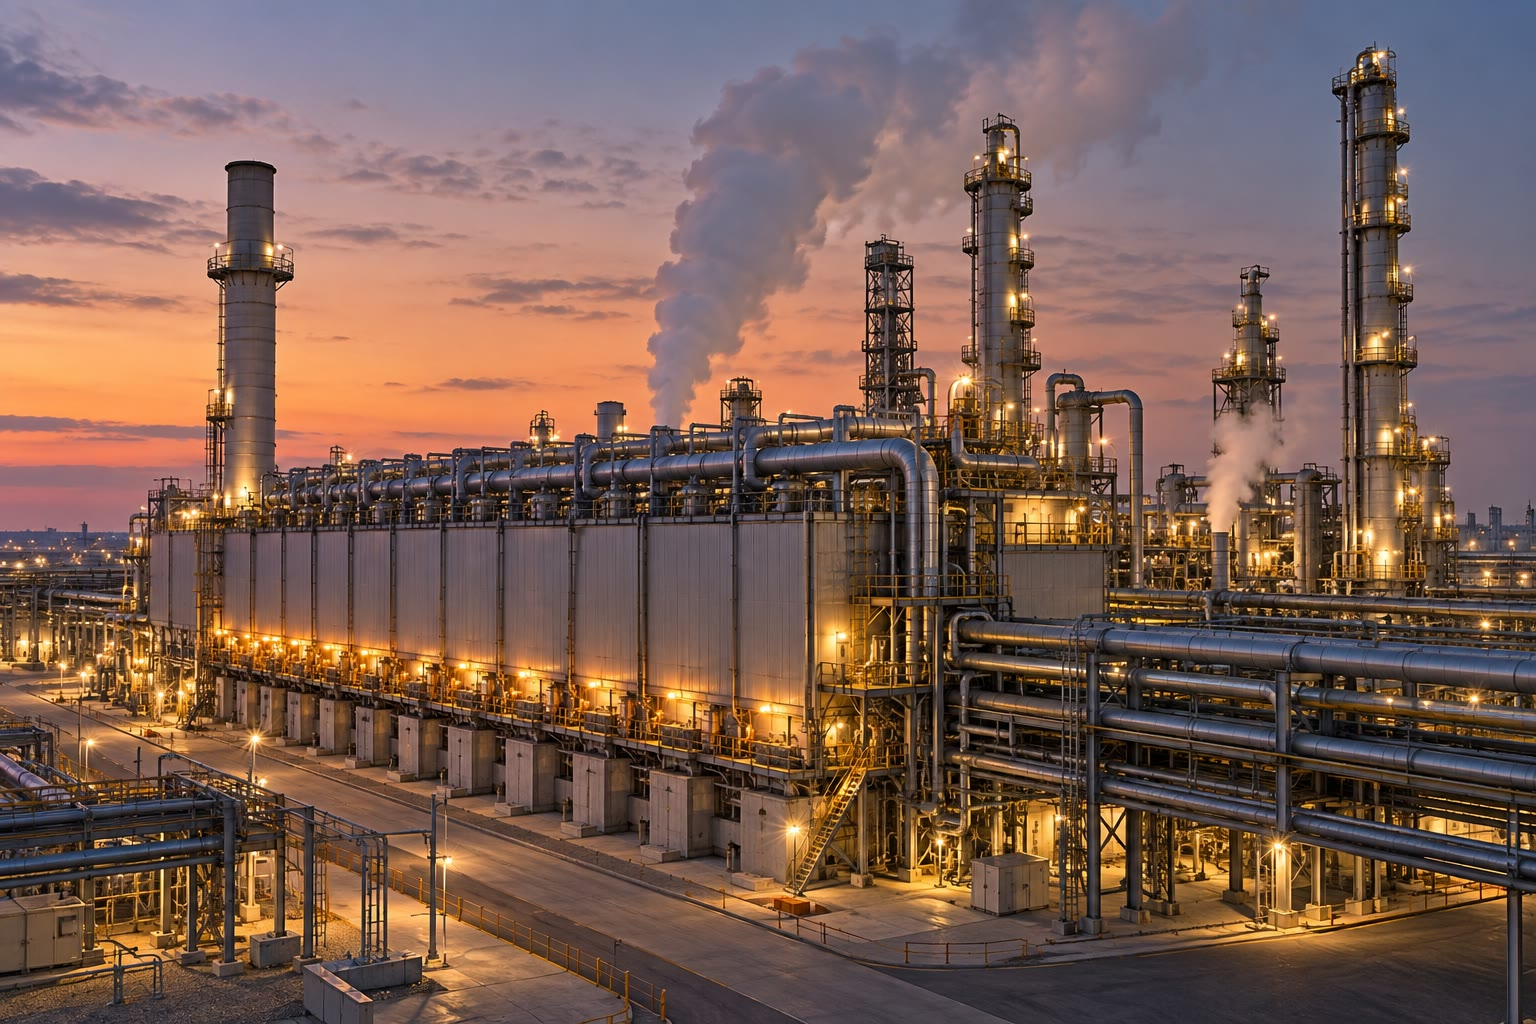
\includegraphics[width=0.6\linewidth]{images/book2/ai/b1-07-hydrogen-plant.jpg}

{\small Sebuah pabrik hidrogen saat senja. Gas alam dan uap air bereaksi
di dalam tungku reformer yang panjang; reaktor kedua mengubah karbon
monoksida; komposisi keluarannya adalah keadaan akhir jenis yang
dihitung dalam bab ini.}
\end{omfigure}

\section{Memerikan sebuah sistem}

\begin{definition}[Sistem, fase]\label{def:b1:extent-q-and-k:system}
\emph{Sistem fisikokimia}\index{sistem fisikokimia} adalah materi yang
terdapat di dalam suatu daerah ruang yang dipilih, sedangkan sisanya
adalah lingkungannya. Sistem itu disebut \emph{sistem
tertutup}\index{sistem tertutup} jika tidak mempertukarkan materi dengan
lingkungannya (sistem itu boleh mempertukarkan energi). \emph{Fase}\index{fase}
adalah bagian sistem yang variabel-variabel \omterm{def:b1:extent-q-and-k:variables}{intensifnya} berubah secara
kontinu: campuran gas adalah satu fase, dua zat cair yang tidak \omterm{def:b1:intermolecular-forces-solvents:miscibility}{dapat
bercampur} adalah dua fase, dan setiap padatan adalah satu fase
tersendiri.
\end{definition}

\begin{definition}[Variabel intensif dan ekstensif]\label{def:b1:extent-q-and-k:variables}
Sebuah variabel keadaan disebut \emph{ekstensif}\index{variabel ekstensif}
jika sebanding dengan ukuran sistem (massa, volume, jumlah zat) dan
\emph{intensif}\index{variabel intensif} jika tidak (suhu, tekanan,
konsentrasi, massa jenis, \omterm{def:b1:extent-q-and-k:composition}{fraksi mol}). Rasio dua variabel ekstensif
bersifat intensif.
\end{definition}

\begin{definition}[Variabel komposisi]\label{def:b1:extent-q-and-k:composition}
Untuk konstituen $i$ sebuah \omterm{def:b1:extent-q-and-k:system}{fase} yang memuat jumlah $n_j$ semua
konstituennya:
\begin{itemize}
  \item \emph{fraksi mol}\index{fraksi mol} konstituen itu adalah $x_i = n_i/\sum_j
        n_j$, dan \emph{fraksi massa}\index{fraksi massa} konstituen itu $w_i =
        m_i/\sum_j m_j$; keduanya terletak antara 0 dan 1 dan berjumlah 1;
  \item dalam larutan bervolume $V$, \emph{konsentrasi
        molar}\index{konsentrasi molar} konstituen itu adalah $c_i = [i] = n_i/V$,
        dalam \unit{mol/L};
  \item dalam campuran gas bertekanan total $p$, \emph{tekanan
        parsial}\index{tekanan parsial} konstituen itu adalah $p_i = x_i\,p$.
\end{itemize}
\end{definition}

\begin{proposition}[Tekanan parsial gas sempurna]\label{prop:b1:extent-q-and-k:dalton}
Dalam campuran gas sempurna bervolume $V$ pada suhu $T$, \omterm{def:b1:extent-q-and-k:composition}{tekanan parsial}
sebuah konstituen adalah tekanan yang akan diberikannya seandainya
konstituen itu sendirian menempati seluruh volume, $p_i = n_iRT/V$, dan
jumlah tekanan-tekanan parsial sama dengan tekanan total: $\sum_i p_i = p$.
\end{proposition}

\begin{proof}
Untuk campuran itu $pV = (\sum_j n_j)RT$, sehingga $p_i = x_i p = \frac{n_i}{\sum_j
n_j}\cdot\frac{(\sum_j n_j)RT}{V} = \frac{n_iRT}{V}$, dan $\sum_i x_i = 1$
menghasilkan $\sum_i p_i = p$.
\end{proof}

\begin{example}[Udara]\label{ex:b1:extent-q-and-k:air}
Udara kering mengandung, menurut volume (yaitu menurut jumlah zat, untuk
gas sempurna), 78.08\,\% dinitrogen, 20.95\,\% dioksigen, dan 0.93\,\%
argon. Pada \qty{1.013}{bar} \omterm{def:b1:extent-q-and-k:composition}{tekanan parsial} dioksigen adalah $0.2095 \times
1.013 = \qty{0.212}{bar}$; di sebuah gunung yang tekanannya
\qty{0.70}{bar}, \omterm{def:b1:extent-q-and-k:composition}{tekanan parsial} itu turun menjadi \qty{0.147}{bar},
walaupun komposisinya sama.
% ledger: air:N2, air:O2, air:Ar, const:atm
\end{example}

\section{Kemajuan reaksi}

\begin{definition}[Bilangan stoikiometri, kemajuan reaksi]\label{def:b1:extent-q-and-k:extent}
Sebuah reaksi ditulis $0 = \sum_i \nu_i\,\mathrm{A}_i$, dengan
\emph{bilangan stoikiometri}\index{bilangan stoikiometri} $\nu_i$ spesies
$\mathrm{A}_i$ bernilai negatif untuk pereaksi dan positif untuk produk:
dalam \ce{N2 + 3H2 -> 2NH3}, $\nu(\ce{N2}) = -1$, $\nu(\ce{H2}) = -3$,
$\nu(\ce{NH3}) = +2$. Dalam \omterm{def:b1:extent-q-and-k:system}{sistem tertutup} yang di dalamnya hanya reaksi
ini yang berlangsung, jumlah-jumlah zat berubah menurut
\[
  n_i = n_{i,0} + \nu_i\,\xi ,
\]
yang mendefinisikan \emph{kemajuan reaksi}\index{kemajuan reaksi}
$\xi$ (dalam mol), nol pada awalnya dan sama untuk setiap spesies.
\end{definition}

\begin{definition}[Kemajuan maksimum, pereaksi pembatas]\label{def:b1:extent-q-and-k:max-extent}
\emph{Kemajuan maksimum}\index{kemajuan maksimum} $\xi_{\max}$ adalah
nilai $\xi$ terbesar yang tidak membuat satu jumlah zat pun negatif: $\xi_{\max} = \min_{\nu_i <
0} n_{i,0}/|\nu_i|$. Pereaksi yang mencapai nol pada $\xi_{\max}$ adalah
\emph{pereaksi pembatas}\index{pereaksi pembatas}. Jika \omterm{def:b1:extent-q-and-k:extent}{kemajuan reaksi}
juga dapat bernilai negatif (reaksi balik), $\xi_{\min} = -\min_{\nu_i > 0}
n_{i,0}/\nu_i$.
\end{definition}

\begin{method}[Tabel kemajuan]\label{met:b1:extent-q-and-k:progress-table}
Untuk mengikuti sebuah reaksi dalam \omterm{def:b1:extent-q-and-k:system}{sistem tertutup}:
\begin{enumerate}
  \item tuliskan persamaan reaksi yang setara, dan di bawahnya satu kolom
        untuk setiap spesies;
  \item baris pertama: jumlah awal $n_{i,0}$;
  \item baris kedua: jumlah pada kemajuan $\xi$, $n_{i,0} + \nu_i\xi$;
  \item untuk gas, tambahkan kolom jumlah total $n_{\text{tot}}(\xi)$;
  \item hitunglah $\xi_{\max}$ (dan $\xi_{\min}$) lalu tentukan \omterm{def:b1:extent-q-and-k:max-extent}{pereaksi
        pembatasnya};
  \item baris terakhir: jumlah akhir, pada kemajuan akhir $\xi_f$ (yang
        diperoleh dari syarat kesetimbangan, atau sama dengan $\xi_{\max}$
        jika reaksinya tuntas).
\end{enumerate}
\end{method}

\begin{example}[Sintesis amonia]\label{ex:b1:extent-q-and-k:ammonia}
Dari \qty{2.0}{mol} \ce{N2} dan \qty{3.0}{mol} \ce{H2}:
\begin{center}
\begin{tabular}{lcccc}
\hline
 & \ce{N2} & \ce{3H2} & \ce{2NH3} & total \\
\hline
awal & 2.0 & 3.0 & 0 & 5.0 \\
kemajuan $\xi$ & $2.0 - \xi$ & $3.0 - 3\xi$ & $2\xi$ & $5.0 - 2\xi$ \\
\hline
\end{tabular}
\end{center}
$\xi_{\max} = \min(2.0/1,\ 3.0/3) = \qty{1.0}{mol}$: dihidrogen adalah
\omterm{def:b1:extent-q-and-k:max-extent}{pereaksi pembatas}. Seandainya reaksinya tuntas, keadaan akhirnya memuat
\qty{1.0}{mol} \ce{N2} dan \qty{2.0}{mol} \ce{NH3}.
\end{example}

\begin{definition}[Rasio kemajuan akhir, rendemen]\label{def:b1:extent-q-and-k:fractional-extent}
\emph{Rasio kemajuan akhir}\index{rasio kemajuan akhir} sebuah reaksi
adalah $\tau = \xi_f/\xi_{\max}$, antara 0 dan 1. Dalam sebuah sintesis,
\emph{rendemen}\index{rendemen} sebuah produk adalah rasio jumlah yang
diperoleh terhadap jumlah yang akan dihasilkan \omterm{def:b1:extent-q-and-k:max-extent}{pereaksi pembatas}
seandainya reaksinya tuntas; jika produk tidak hilang selama isolasi,
rendemen sama dengan $\tau$.
\end{definition}

\section{Aktivitas}

\begin{definition}[Keadaan standar, aktivitas]\label{def:b1:extent-q-and-k:activity}
\emph{Aktivitas}\index{aktivitas} $a_i$ sebuah spesies adalah bilangan
tak berdimensi yang mengukur, dalam ungkapan hukum-hukum kesetimbangan,
seberapa banyak spesies itu tersedia; aktivitas didefinisikan relatif
terhadap sebuah \emph{keadaan standar}\index{keadaan standar}, yaitu
keadaan acuan pada suhu yang ditinjau dan pada tekanan standar
$p^\circ = \qty{1}{bar}$. Dalam pendekatan-pendekatan ideal yang dipakai
dalam buku ini:
\begin{itemize}
  \item untuk gas, $a_i = p_i/p^\circ$ (keadaan standarnya adalah gas
        sempurna murni pada $p^\circ$);
  \item untuk zat terlarut dalam larutan encer, $a_i = c_i/c^\circ$
        dengan $c^\circ = \qty{1}{mol/L}$;
  \item untuk pelarut larutan encer, dan untuk padatan murni atau zat
        cair murni yang sendirian dalam \omterm{def:b1:extent-q-and-k:system}{fasenya}, $a_i = 1$.
\end{itemize}
\end{definition}
% ledger: const:pstd

\begin{remark}[Ideal dan nyata]\label{rem:b1:extent-q-and-k:ideal}
Ungkapan-ungkapan ini berlaku untuk gas sempurna dan untuk larutan encer.
Dalam larutan pekat ion-ion saling tarik dan saling tolak, dan
\omterm{def:b1:extent-q-and-k:activity}{aktivitasnya} menyimpang dari $c_i/c^\circ$; koreksinya, yang ditulis
dengan koefisien \omterm{def:b1:extent-q-and-k:activity}{aktivitas}, dipelajari dalam jilid Tahun 2 bersama
potensial kimia. Untuk konsentrasi yang dipakai dalam buku ini (di bawah
sekitar \qty{0.1}{mol/L}) ungkapan ideal akurat sampai beberapa persen.
\end{remark}

\section{Kuosien reaksi dan tetapan kesetimbangan}

\begin{definition}[Kuosien reaksi]\label{def:b1:extent-q-and-k:quotient}
\emph{Kuosien reaksi}\index{kuosien reaksi} sebuah reaksi
$0 = \sum_i \nu_i\,\mathrm{A}_i$ pada suatu keadaan sistem adalah
\[
  Q = \prod_i a_i^{\nu_i} ,
\]
yaitu hasil kali \omterm{def:b1:extent-q-and-k:activity}{aktivitas} produk dibagi dengan hasil kali \omterm{def:b1:extent-q-and-k:activity}{aktivitas}
pereaksi, masing-masing dipangkatkan dengan koefisien stoikiometrinya.
\end{definition}

\begin{example}[Tiga kuosien]\label{ex:b1:extent-q-and-k:quotients}
Untuk \ce{N2(g) + 3H2(g) <=> 2NH3(g)}: $Q = \dfrac{(p_{\ce{NH3}}/p^\circ)^2}
{(p_{\ce{N2}}/p^\circ)(p_{\ce{H2}}/p^\circ)^3}$. Untuk
\ce{CH3COOH(aq) + H2O(l) <=> CH3COO^-(aq) + H3O+(aq)}: $Q =
\dfrac{[\ce{CH3COO-}][\ce{H3O+}]}{[\ce{CH3COOH}]\,c^\circ}$, karena
\omterm{def:b1:extent-q-and-k:activity}{aktivitas} pelarutnya 1. Untuk \ce{CaCO3(s) <=> CaO(s) + CO2(g)}: $Q =
p_{\ce{CO2}}/p^\circ$, karena \omterm{def:b1:extent-q-and-k:activity}{aktivitas} padatan-padatannya 1.
\end{example}

\begin{definition}[Tetapan kesetimbangan standar]\label{def:b1:extent-q-and-k:equilibrium-constant}
\emph{Tetapan kesetimbangan standar}\index{tetapan kesetimbangan standar}
$K^\circ$ sebuah reaksi adalah nilai yang diambil oleh \omterm{def:b1:extent-q-and-k:quotient}{kuosien reaksinya}
ketika sistem berada dalam kesetimbangan. Tetapan ini tak berdimensi dan
hanya bergantung pada reaksi dan suhu.
\end{definition}

\begin{theorem}[Hukum aksi massa]\label{thm:b1:extent-q-and-k:mass-action}
Pada suhu tertentu, sistem yang di dalamnya sebuah reaksi dapat
berlangsung ke kedua arah berevolusi sampai $Q = K^\circ(T)$; pada
kesetimbangan, apa pun komposisi awalnya,
\[
  \prod_i a_{i,\text{eq}}^{\nu_i} = K^\circ(T) .
\]
\end{theorem}
\admitted

\begin{proposition}[Arah evolusi]\label{prop:b1:extent-q-and-k:direction}
Sistem dengan $Q < K^\circ$ berevolusi ke arah maju ($\xi$ bertambah);
jika $Q > K^\circ$, sistem berevolusi ke arah balik; jika $Q = K^\circ$,
sistem berada dalam kesetimbangan.
\end{proposition}
\admitted

\begin{remark}[Asal hukum-hukum ini]\label{rem:b1:extent-q-and-k:origin}
Kedua pernyataan itu diturunkan dari hukum kedua termodinamika, melalui
energi bebas reaksi dan potensial kimia spesies-spesiesnya: keduanya
diturunkan dalam jilid Tahun 2, yang juga memberikan $K^\circ$ dari tabel
data termodinamika dan menjelaskan bagaimana tetapan itu berubah dengan
suhu. Di sini keduanya dipakai sebagai hukum.
\end{remark}

\begin{omfigure}
\begin{tikzpicture}[font=\small, >={Stealth}]
  \draw[->, thick] (0,0) -- (11,0) node[right] {$Q$};
  \draw[thick, omThm] (5.5,0.25) -- (5.5,-0.25) node[below] {$K^\circ$};
  \draw[->, omDef, thick] (1.0,0.55) -- (4.6,0.55);
  \node[above, omDef] at (2.8,0.6) {$Q < K^\circ$: maju};
  \draw[->, omProp, thick] (10.0,0.55) -- (6.4,0.55);
  \node[above, omProp] at (8.2,0.6) {$Q > K^\circ$: balik};
  \node[below] at (0,-0.1) {0};
\end{tikzpicture}

{\small Kuosien bergerak menuju tetapan: sistem dengan $Q <
K^\circ$ menghasilkan produk, sistem dengan $Q > K^\circ$ mengonsumsinya.}
\end{omfigure}

\begin{proposition}[Menggabungkan tetapan]\label{prop:b1:extent-q-and-k:combine-k}
Jika $K_1^\circ$ dan $K_2^\circ$ adalah tetapan reaksi (1) dan (2):
kebalikan reaksi (1) mempunyai tetapan $1/K_1^\circ$; reaksi $n \times
(1)$ mempunyai $(K_1^\circ)^n$; jumlah $(1) + (2)$ mempunyai $K_1^\circ K_2^\circ$.
\end{proposition}

\begin{proof}
\omterm{def:b1:extent-q-and-k:quotient}{Kuosien reaksi} balik adalah $\prod a_i^{-\nu_i} = 1/Q_1$; kuosien
$n \times (1)$ adalah $\prod a_i^{n\nu_i} = Q_1^n$; kuosien jumlahnya adalah
$\prod a_i^{\nu_{i,1} + \nu_{i,2}} = Q_1 Q_2$. Dengan menuliskan
identitas-identitas ini pada kesetimbangan, ketika setiap kuosien sama
dengan tetapannya, diperoleh hasil tersebut.
\end{proof}

\begin{proposition}[Satu keadaan kesetimbangan]\label{prop:b1:extent-q-and-k:q-monotone}
Untuk satu reaksi dalam \omterm{def:b1:extent-q-and-k:system}{sistem tertutup} pada suhu tetap (dan, untuk gas,
pada volume atau tekanan tetap), kuosien $Q(\xi)$ adalah fungsi $\xi$
yang naik tegas pada $(\xi_{\min}, \xi_{\max})$, dari 0 sampai $+\infty$
jika tidak ada spesies beraktivitas tetap yang terlibat. Maka persamaan
$Q(\xi) = K^\circ$ mempunyai tepat satu penyelesaian pada selang ini.
\end{proposition}

\begin{proof}
Tinjau reaksi dalam larutan, $Q(\xi) = \prod_i (n_{i,0} + \nu_i\xi)^{\nu_i}
\times \text{tetapan}$. Turunan logaritmiknya adalah
\[
  \frac{\dd \ln Q}{\dd \xi} = \sum_i \frac{\nu_i^2}{n_{i,0} + \nu_i \xi}
  > 0 ,
\]
dengan setiap suku positif di daerah tempat semua jumlah zat positif.
Ketika $\xi \to \xi_{\max}$ jumlah salah satu pereaksi menuju 0 pada
sebuah penyebut dan $Q \to +\infty$; ketika $\xi
\to \xi_{\min}$ jumlah salah satu produk menuju 0 dan $Q \to 0$. Fungsi
naik yang kontinu dari 0 sampai $+\infty$ mengambil nilai $K^\circ$ satu
kali. (Untuk gas pada tekanan tetap, jumlah totalnya juga berubah; hasil
itu tetap berlaku, sebagaimana dapat diperiksa dalam setiap kasus.)
\end{proof}

\section{Keadaan akhir}

\begin{definition}[Keadaan kesetimbangan, reaksi kuantitatif]\label{def:b1:extent-q-and-k:quantitative}
Keadaan akhir adalah
\emph{keadaan kesetimbangan}\index{keadaan kesetimbangan} jika semua spesies reaksi hadir dan $Q = K^\circ$. Reaksi
itu \emph{kuantitatif}\index{reaksi kuantitatif} (atau tuntas) jika pada
keadaan akhir \omterm{def:b1:extent-q-and-k:max-extent}{pereaksi pembatasnya} praktis telah habis,
$\xi_f \approx \xi_{\max}$; hal ini terjadi jika $K^\circ$ sangat besar.
\end{definition}

\begin{method}[Menentukan keadaan akhir]\label{met:b1:extent-q-and-k:final-state}
Untuk menentukan keadaan akhir satu reaksi:
\begin{enumerate}
  \item gambarlah tabel kemajuan dan hitunglah $\xi_{\max}$ (dan
        $\xi_{\min}$);
  \item hitunglah $Q$ pada awalnya dan bandingkan dengan $K^\circ$ untuk
        menentukan arahnya;
  \item nyatakan $Q(\xi)$ dengan \omterm{def:b1:extent-q-and-k:activity}{aktivitas-aktivitasnya} lalu selesaikan
        $Q(\xi) = K^\circ$ untuk $\xi$ pada $(\xi_{\min}, \xi_{\max})$;
  \item jika sebuah spesies beraktivitas 1 (sebuah padatan) terlibat,
        periksalah bahwa spesies itu masih ada pada kemajuan tersebut:
        jika jumlahnya harus menjadi negatif, spesies itu habis lebih
        dahulu dan keadaan akhirnya \emph{bukan} kesetimbangan
        ($\xi_f = \xi_{\max}$, $Q_f \ne K^\circ$).
\end{enumerate}
\end{method}

\begin{method}[Hipotesis reaksi kuantitatif]\label{met:b1:extent-q-and-k:quantitative}
Jika $K^\circ$ besar (biasanya di atas $10^4$), anggaplah reaksinya
tuntas: tetapkan $\xi_f = \xi_{\max}$, hitunglah jumlah-jumlah akhirnya,
lalu tentukan jumlah kecil $\varepsilon$ \omterm{def:b1:extent-q-and-k:max-extent}{pereaksi pembatas} yang tersisa
dengan menuliskan $Q =
K^\circ$ sementara jumlah-jumlah lainnya tidak
berubah. Hipotesis itu diterima jika $\varepsilon$ kecil dibandingkan
dengan jumlah-jumlah lainnya (di bawah sekitar 1\,\%).
\end{method}

\begin{example}[Sebuah reaksi kuantitatif]\label{ex:b1:extent-q-and-k:quant}
Untuk $\mathrm{A + B \rightleftharpoons C + D}$ dalam larutan dengan $[\ce{A}]_0 = [\ce{B}]_0 =
\qty{0.10}{mol/L}$ dan $K^\circ = 10^6$: dengan menganggap reaksinya
tuntas, $[\ce{C}]
= [\ce{D}] = 0.10$; lalu $0.10^2/\varepsilon^2 = 10^6$ menghasilkan $\varepsilon
= \qty{1.0e-4}{mol/L}$, 0.1\,\% dari jumlah awal: hipotesis itu sahih.
\end{example}

\begin{omfigure}
\begin{tikzpicture}
\begin{axis}[
  width=0.45\linewidth, height=5.6cm, ymode=log,
  xmin=0, xmax=1, ymin=0.01, ymax=1000,
  axis x line=bottom, axis y line=left,
  xlabel={kemajuan $\xi$ (mol)}, ylabel={$Q$}, xtick={0,0.2,0.4,0.8,1},
  tick label style={font=\small}, label style={font=\small}, clip=false]
\addplot[omDef, thick] table[x=xi, y=Q] {figdata/out/bachelor-1-extent-equilibrium-shift.dat};
\draw[omThm, dashed] (axis cs:0,4) -- (axis cs:1,4);
\node[omThm, anchor=south west, font=\small] at (axis cs:0.02,4) {$K^\circ = 4.0$};
\draw[dotted] (axis cs:0.607,0.01) -- (axis cs:0.607,4);
\node[anchor=north, font=\small] at (axis cs:0.607,0.01) {0.607};
\end{axis}
\end{tikzpicture}\hfill
\begin{tikzpicture}
\begin{axis}[
  width=0.45\linewidth, height=5.6cm,
  xmin=0, xmax=0.04, ymin=0, ymax=0.3,
  axis x line=bottom, axis y line=left,
  xlabel={kemajuan $\xi$ (mol)}, ylabel={$Q = p_{\ce{CO2}}/p^\circ$},
  xtick={0,0.01,0.02,0.03,0.04}, scaled x ticks=false,
  xticklabel style={/pgf/number format/fixed, /pgf/number format/precision=2},
  yticklabel style={/pgf/number format/fixed},
  tick label style={font=\small}, label style={font=\small}, clip=false]
\addplot[omProp, thick] table[x=xi, y=Q_small] {figdata/out/bachelor-1-extent-equilibrium-carbonate.dat};
\addplot[omDef, thick, dashed] table[x=xi, y=Q_large] {figdata/out/bachelor-1-extent-equilibrium-carbonate.dat};
\draw[omThm, dashed] (axis cs:0,0.2) -- (axis cs:0.04,0.2);
\node[omThm, anchor=south west, font=\small] at (axis cs:0.0005,0.2) {$K^\circ = 0.20$};
\node[omProp, anchor=north west, font=\scriptsize] at (axis cs:0.012,0.088) {\qty{0.010}{mol}: padatan habis};
\node[omDef, anchor=north west, font=\scriptsize] at (axis cs:0.024,0.19) {\qty{0.050}{mol}: kesetimbangan};
\end{axis}
\end{tikzpicture}

{\small Kiri: kuosien \ce{CO + H2O <=> CO2 + H2} naik seiring \omterm{def:b1:extent-q-and-k:extent}{kemajuan
reaksi} dan bertemu $K^\circ$ satu kali (soal akhir pekan). Kanan: untuk
\ce{CaCO3(s) <=> CaO(s) + CO2(g)} dalam bejana tertutup \qty{10}{L},
$Q = p_{\ce{CO2}}/p^\circ$ bertambah dengan $\xi$; dengan \qty{0.050}{mol}
karbonat kuosien itu mencapai $K^\circ = 0.20$ (kesetimbangan), dengan
\qty{0.010}{mol} karbonatnya habis lebih dahulu dan keadaan akhirnya
bukan kesetimbangan.}
\end{omfigure}

\begin{method}[Dua reaksi serentak]\label{met:b1:extent-q-and-k:two-reactions}
Jika dua reaksi berlangsung dalam sistem yang sama, berilah masing-masing
\omterm{def:b1:extent-q-and-k:extent}{kemajuan reaksinya} sendiri, $\xi_1$ dan $\xi_2$; setiap jumlah zat adalah
$n_i = n_{i,0} + \nu_{i,1}\xi_1
+ \nu_{i,2}\xi_2$, dan keadaan akhirnya memenuhi $Q_1 = K_1^\circ$ dan
sekaligus $Q_2 = K_2^\circ$ (sistem dua persamaan). Jika satu tetapan jauh
lebih besar daripada yang lain, perlakukan reaksi yang bersangkutan lebih
dahulu sebagai \omterm{def:b1:extent-q-and-k:quantitative}{reaksi kuantitatif}, lalu reaksi kedua pada hasilnya.
\end{method}

\begin{history}[Hukum aksi massa, 1864]
Pada tahun 1864 ahli kimia Norwegia Cato Guldberg dan iparnya, apoteker
Peter Waage, menerbitkan dalam bahasa Norwegia hukum ``massa aktif''
mereka: sebuah reaksi berlangsung sampai gaya reaksi maju dan reaksi
balik seimbang, masing-masing sebanding dengan konsentrasi
pereaksi-pereaksinya. Karya mereka tidak diperhatikan di luar negeri
sampai mereka menerbitkannya kembali dalam dua bahasa yang lebih luas
dibaca, pada tahun 1867 dan 1879; Jacobus van 't Hoff, yang menemukan
kembali hukum itu, mengakui keutamaan mereka.
\end{history}

\section{Latihan}

\begin{exercise}[$\star$]\label{exo:b1:extent-q-and-k:1}
Golongkan sebagai \omterm{def:b1:extent-q-and-k:variables}{intensif} atau \omterm{def:b1:extent-q-and-k:variables}{ekstensif}: suhu, volume, jumlah zat,
\omterm{def:b1:extent-q-and-k:composition}{konsentrasi molar}, massa jenis, tekanan, massa, \omterm{def:b1:extent-q-and-k:composition}{fraksi mol}.
\end{exercise}

\begin{exercise}[$\star$]\label{exo:b1:extent-q-and-k:2}
Dengan komposisi udara kering yang diberikan dalam bab ini, hitunglah
\omterm{def:b1:extent-q-and-k:composition}{tekanan parsial} \ce{N2}, \ce{O2}, dan \ce{Ar} pada tekanan total
\qty{1.013}{bar}.
\end{exercise}

\begin{exercise}[$\star$]\label{exo:b1:extent-q-and-k:3}
Gambarlah tabel kemajuan \ce{2H2 + O2 -> 2H2O} dari \qty{3.0}{mol}
\ce{H2} dan \qty{2.0}{mol} \ce{O2}. Tentukan $\xi_{\max}$, \omterm{def:b1:extent-q-and-k:max-extent}{pereaksi
pembatas}, dan keadaan akhirnya jika reaksinya tuntas.
\end{exercise}

\begin{exercise}[$\star$]\label{exo:b1:extent-q-and-k:4}
Tuliskan \omterm{def:b1:extent-q-and-k:quotient}{kuosien reaksi}: (a) \ce{CaCO3(s) <=> CaO(s) + CO2(g)};
(b) \ce{Ag+(aq) + Cl-(aq) <=> AgCl(s)}; (c) \ce{N2(g) + 3H2(g) <=>
2NH3(g)}; (d) \ce{NH3(aq) + H2O(l) <=> NH4+(aq) + OH-(aq)}.
\end{exercise}

\begin{exercise}[$\star\star$]\label{exo:b1:extent-q-and-k:5}
Reaksi (1) $\mathrm{A \rightleftharpoons B}$ dan (2) $\mathrm{B \rightleftharpoons C}$ mempunyai tetapan
$K_1^\circ = 10$ dan $K_2^\circ = 0.5$. Tentukan tetapan $\mathrm{A \rightleftharpoons C}$,
$\mathrm{C \rightleftharpoons A}$, dan $\mathrm{2\,A \rightleftharpoons 2\,C}$.
\end{exercise}

\begin{exercise}[$\star\star$]\label{exo:b1:extent-q-and-k:6}
Sebuah reaksi mempunyai $K^\circ = 2.0 \times 10^{-3}$. Ke arah manakah
sistem berevolusi jika, pada awalnya, $Q = 5.0 \times 10^{-5}$? Jika
$Q = 0.10$? Jika hanya ada pereaksi?
\end{exercise}

\begin{exercise}[$\star\star$]\label{exo:b1:extent-q-and-k:7}
Gas \ce{A2} terdisosiasi, \ce{A2(g) <=> 2A(g)}, dengan $K^\circ = 0.25$
pada suhu percobaan. Mulai dari \qty{1.0}{mol} \ce{A2} pada tekanan total
yang dijaga tetap $p^\circ$, tuliskan tabel kemajuan beserta jumlah
totalnya, nyatakan $Q(\xi)$, lalu tentukan kemajuan kesetimbangannya.
\end{exercise}

\begin{exercise}[$\star\star$]\label{exo:b1:extent-q-and-k:8}
Dalam larutan, $\mathrm{A + B \rightleftharpoons C}$ dengan $K^\circ = 100$ dan konsentrasi
awal $[\ce{A}]_0 = [\ce{B}]_0 = \qty{0.10}{mol/L}$. Tentukan konsentrasi
kesetimbangan dan \omterm{def:b1:extent-q-and-k:fractional-extent}{rasio kemajuan akhirnya}.
\end{exercise}

\begin{exercise}[$\star\star$]\label{exo:b1:extent-q-and-k:9}
Untuk $\mathrm{A + B \rightleftharpoons C + D}$ dari jumlah \ce{A} dan \ce{B} yang sama,
tunjukkan bahwa \omterm{def:b1:extent-q-and-k:fractional-extent}{rasio kemajuan akhirnya} adalah
$\tau = \sqrt{K^\circ}/(1 + \sqrt{K^\circ})$.
Berapa nilai $K^\circ$ yang menghasilkan $\tau = 0.99$?
\end{exercise}

\begin{exercise}[$\star\star\star$]\label{exo:b1:extent-q-and-k:10}
Kalsium karbonat dipanaskan pada \qty{1100}{K} dalam bejana tertutup
\qty{10.0}{L}, yang pada awalnya kosong dari gas, dengan $K^\circ = 0.20$
untuk \ce{CaCO3(s) <=> CaO(s) + CO2(g)}. Tentukan keadaan akhirnya untuk
\qty{0.010}{mol} dan untuk \qty{0.050}{mol} karbonat.
\end{exercise}

\begin{exercise}[$\star\star\star$]\label{exo:b1:extent-q-and-k:11}
Sebuah zat \ce{A} berisomerisasi dalam larutan melalui dua cara,
$\mathrm{A \rightleftharpoons B}$
($K_1^\circ = 2.0$) dan $\mathrm{A \rightleftharpoons C}$ ($K_2^\circ = 3.0$). Mulai dari
\qty{1.0}{mol} \ce{A} saja, tentukan jumlah akhir ketiga isomer itu.
\end{exercise}

\begin{exercise}[$\star\star\star$]\label{exo:b1:extent-q-and-k:12}
Sebuah asam \ce{A} dan sebuah alkohol \ce{B} menghasilkan ester dan air,
$\mathrm{A + B
\rightleftharpoons E + W}$, semuanya dalam satu \omterm{def:b1:extent-q-and-k:system}{fase} cair, dengan $K^\circ = 4.0$
(ambillah \omterm{def:b1:extent-q-and-k:activity}{aktivitas} sama dengan \omterm{def:b1:extent-q-and-k:composition}{fraksi mol}; jumlah totalnya tidak
berubah). Hitunglah \omterm{def:b1:extent-q-and-k:fractional-extent}{rendemen} maksimum ester dari \qty{0.50}{mol} setiap
pereaksi, lalu dari \qty{0.50}{mol} asam dan \qty{1.0}{mol} alkohol.
\end{exercise}

\section{Soal: Keluaran Sebuah Pabrik Hidrogen}

\begin{problem}[{Soal akhir pekan --- variabel komposisi umpan,
reformasi kukus yang dianggap tuntas, reaksi geser air--gas pada
kesetimbangan, dan kadar hidrogen gas yang keluar dari pabrik}]
\label{pb:b1:extent-q-and-k:1}
Sebuah pabrik hidrogen diumpani \qty{1.00}{mol} metana dan
\qty{3.00}{mol} uap air (per satuan waktu) pada \qty{30}{bar}. Di dalam
reformer, \ce{CH4 + H2O -> CO + 3H2} dianggap tuntas. Di dalam reaktor
geser, \ce{CO + H2O <=> CO2 + H2} mencapai kesetimbangan; ambillah
$K^\circ =
4.0$ pada suhunya. Massa molar: \ce{CH4} \qty{16.04}{g/mol},
\ce{H2O} \qty{18.02}{g/mol}.

\medskip
\noindent\textbf{Bagian I --- Umpan.}
\begin{enumerate}
  \item Hitunglah \omterm{def:b1:extent-q-and-k:composition}{fraksi mol} metana dan uap air dalam umpan.
  \item Hitunglah \omterm{def:b1:extent-q-and-k:composition}{tekanan parsialnya}.
  \item Hitunglah \omterm{def:b1:extent-q-and-k:composition}{fraksi massanya}.
  \item Besaran-besaran manakah yang sejauh ini dipakai yang bersifat
        \omterm{def:b1:extent-q-and-k:variables}{intensif}?
  \item Tentukan \omterm{def:b1:extent-q-and-k:activity}{aktivitas} metana dan uap air dalam umpan.
\end{enumerate}

\medskip
\noindent\textbf{Bagian II --- Reformasi.}
\begin{enumerate}[resume]
  \item Gambarlah tabel \omterm{def:b1:extent-q-and-k:extent}{kemajuan reaksi} reformasi.
  \item Hitunglah $\xi_{\max}$ dan sebutkan \omterm{def:b1:extent-q-and-k:max-extent}{pereaksi pembatasnya}.
  \item Tentukan jumlah-jumlah yang keluar dari reformer.
  \item Hitunglah jumlah total gas, lalu bandingkan dengan umpan.
  \item Hitunglah \omterm{def:b1:extent-q-and-k:composition}{fraksi mol} yang keluar dari reformer.
  \item Mengapa uap air diumpankan berlebih?
\end{enumerate}

\medskip
\noindent\textbf{Bagian III --- Reaktor geser.}
\begin{enumerate}[resume]
  \item Gambarlah tabel \omterm{def:b1:extent-q-and-k:extent}{kemajuan reaksi} geser, mulai dari gas yang keluar
        dari reformer.
  \item Tunjukkan bahwa $Q(\xi) = \dfrac{\xi(3 + \xi)}{(1 - \xi)(2 - \xi)}$,
        dan bahwa kuosien itu tidak bergantung pada tekanan.
  \item Hitunglah $Q$ di saluran masuk dan ramalkan arah evolusinya.
  \item Tuliskan persamaan untuk kemajuan kesetimbangan lalu
        selesaikanlah, dengan mempertahankan akar yang bermakna.
  \item Tentukan jumlah-jumlah yang keluar dari reaktor geser.
  \item Hitunglah \omterm{def:b1:extent-q-and-k:fractional-extent}{rasio kemajuan akhir} reaksi geser.
  \item Dengan uap air dua kali lebih banyak dalam umpan
        (\qty{6.00}{mol}), gas memasuki reaktor geser dengan
        \qty{5.00}{mol} uap air: hitunglah kemajuan kesetimbangan yang
        baru.
\end{enumerate}

\medskip
\noindent\textbf{Bagian IV --- Yang keluar dari pabrik.}
\begin{enumerate}[resume]
  \item Berapa nilai $K^\circ$ yang diperlukan untuk mengubah 99\,\%
        karbon monoksida pada kasus pertama?
  \item Jelaskan mengapa reaktor geser mengubah lebih banyak jika bekerja
        pada suhu tempat tetapannya lebih besar, dan mengapa pabrik
        memakai dua reaktor geser yang dipasang seri.
  \item Uap air diembunkan dari gas yang keluar dari reaktor geser.
        Hitunglah \omterm{def:b1:extent-q-and-k:composition}{fraksi mol} hidrogen dalam gas kering itu.
  \item Daftarkan pengotor yang tersisa beserta jumlahnya.
  \item Hitunglah \omterm{def:b1:extent-q-and-k:composition}{fraksi mol} hidrogen dalam gas yang keluar dari reaktor
        geser, termasuk uap airnya.
\end{enumerate}
\end{problem}
